\chapter{晶体学与 X 射线衍射}\label{ch:b3:x-ray-diffraction}

1912 年，一束 X 射线穿过硫酸铜晶体，在照相底片上留下了
一组清晰的斑点。晶体衍射 X 射线的方式，与衍射光栅
衍射光的方式相同，原因在于晶体中原子之间的距离
与 X 射线的波长相当。一年后，当时还是学生的威廉·劳伦斯·布拉格
从这类图样中解读出岩盐的结构——并证明
这种固体中并不含 \ce{NaCl} 分子，只有一种点阵，其中每个离子
都有六个异种离子近邻。本书及一年级分册中引用的每一种晶体结构
都是以这种方式得到的。本章介绍点阵的几何及其对称性，
衍射的条件，
揭示晶胞内容的衍射强度，以及
各实验室普遍使用的粉末法和单晶法。

\begin{recall}
一年级分册用结点点阵、基元及带晶格参数的晶胞描述晶体，
计算了晶胞的多重度，构造了面心立方、体心立方和六方密堆积结构，
以及岩盐型、氯化铯型、闪锌矿型
和萤石型结构，并由晶胞算出密度。
\Cref{ch:b3:point-groups}中定义了
\omterm{def:b3:point-groups:operation}{对称操作}和\omterm{def:b3:point-groups:point-group}{点群}。
\end{recall}

\begin{omfigure}
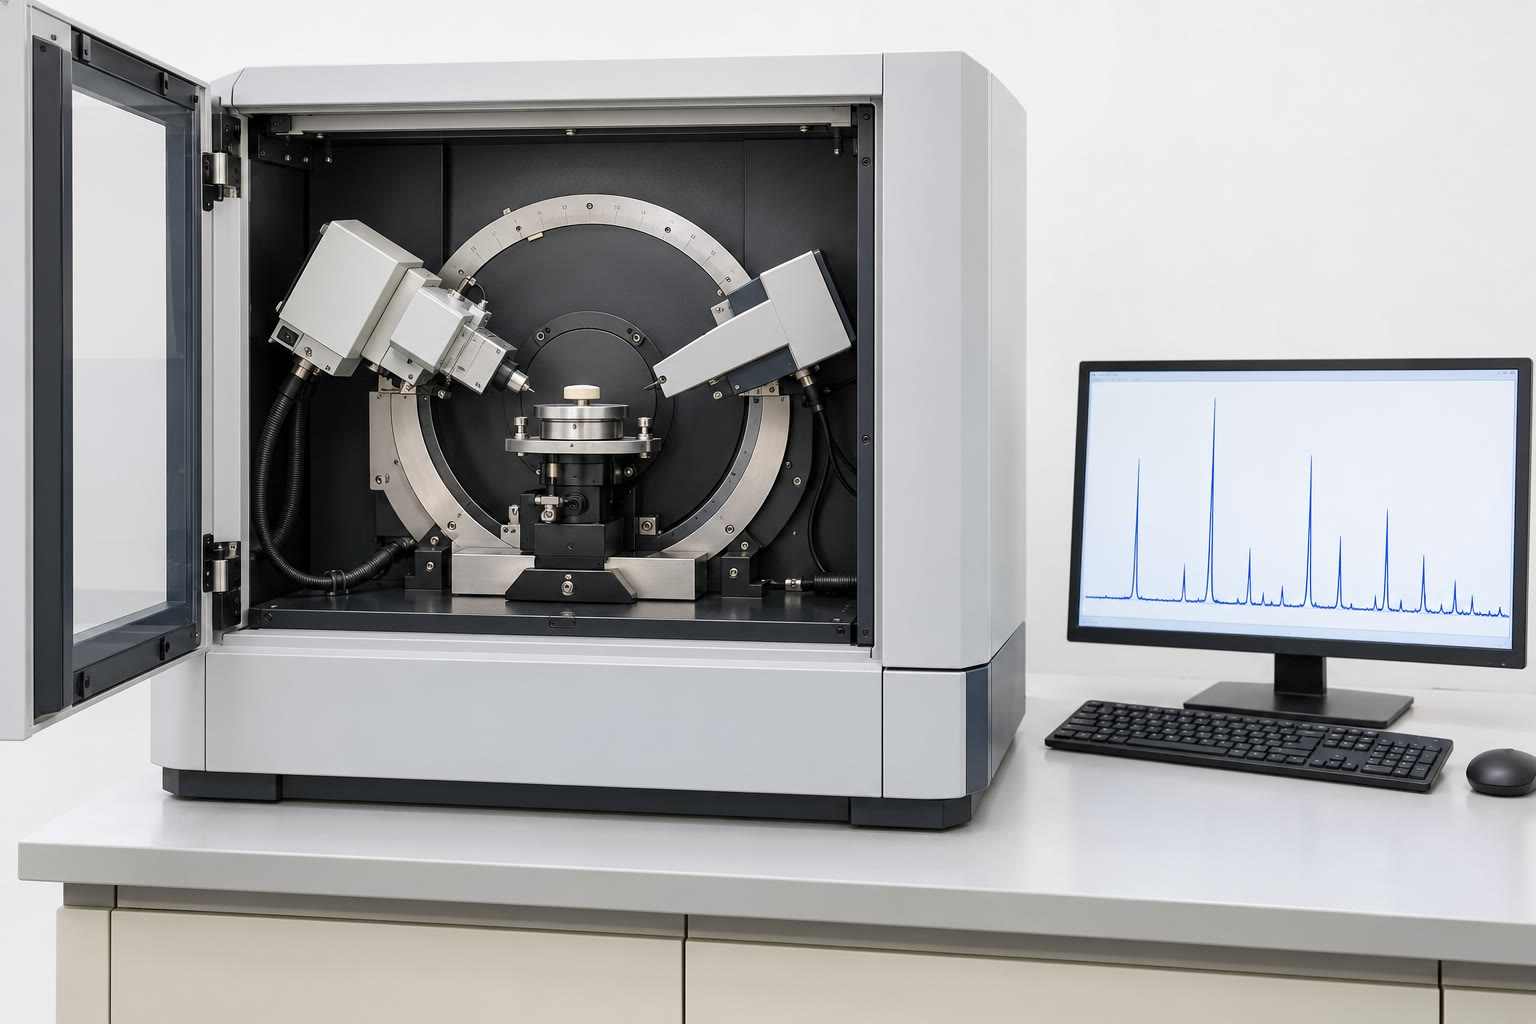
\includegraphics[width=0.6\linewidth]{images/book4/ai/b3-09-diffractometer.jpg}

{\small 台式粉末衍射仪：X 射线管与探测器
绕平板样品在圆周上转动。}
\end{omfigure}

\section{晶系与布拉维点阵}

点阵只能具有把点阵映射到自身上的\omterm{def:b3:point-groups:operation}{对称操作}。
这一限制十分严格。

\begin{theorem}[晶体学限制]\label{thm:b3:x-ray-diffraction:restriction}
与点阵相容的旋转轴只能是 1、2、3、4 和 6 次轴。
\end{theorem}

\begin{proof}
在点阵矢量的基下，对称旋转把点阵矢量映为
点阵矢量，因此其矩阵元素为整数，迹亦为整数。
迹不依赖于基的选取；在沿 $z$ 轴取标准正交基时，迹为
$1 + 2\cos\theta$。于是 $2\cos\theta$ 是介于 $-2$ 与 2 之间的整数：
$\cos\theta \in \{-1, -\frac12, 0, \frac12, 1\}$，$\theta = 180^\circ, 120^\circ, 90^\circ,
60^\circ, 0^\circ$，分别对应 2、3、4、6、1 次轴。五次轴不可能存在。
\end{proof}

\begin{definition}[晶系、布拉维点阵、点阵带心]\label{def:b3:x-ray-diffraction:crystal-system}
按对称性，点阵可分为七种\emph{晶系}\index{晶系}
（三斜、单斜、正交、四方、三方、六方、立方）。
晶胞中的结点可只位于顶角（简单，P），
或另在体心（I）、各面中心（F），
或仅在一对面的中心（底心，C），或沿体对角线（菱方，R）。
这种性质称为
\emph{点阵带心}\index{点阵带心}。晶系与带心的 14 种不同组合，
称为\emph{布拉维点阵}\index{布拉维点阵}。
\end{definition}

\begin{center}\small
\begin{tabular}{lll}
\hline
\omterm{def:b3:x-ray-diffraction:crystal-system}{晶系} & 晶胞约束 & 带心 \\ \hline
三斜 & 无 & P \\
单斜 & $\alpha = \gamma = 90^\circ$ & P, C \\
正交 & $\alpha = \beta = \gamma = 90^\circ$ & P, C, I, F \\
四方 & $a = b$，所有角均为 $90^\circ$ & P, I \\
三方 & $a = b = c$，$\alpha = \beta = \gamma \ne 90^\circ$（菱方轴） & R \\
六方 & $a = b$，$\alpha = \beta = 90^\circ$，$\gamma = 120^\circ$ & P \\
立方 & $a = b = c$，所有角均为 $90^\circ$ & P, I, F \\ \hline
\end{tabular}
\end{center}

\begin{omfigure}
\tdplotsetmaincoords{60}{100}
\begin{tikzpicture}[tdplot_main_coords, scale=1.25, font=\small]
  \foreach \s/\lab in {0/{立方 P}, 3.0/{立方 I}, 6.0/{立方 F}}{
    \begin{scope}[xshift=\s cm]
      \pic[transform shape] {omcubeo={1.6}};
      \foreach \x in {0,1.6}{\foreach \y in {0,1.6}{\foreach \z in {0,1.6}{\node[cellA=2.6mm] at (\x,\y,\z) {};}}}
      \node[anchor=north] at (0.8,0.8,-0.62) {\lab};
    \end{scope}}
  \begin{scope}[xshift=3.0cm]
    \node[cellB=2.6mm] at (0.8,0.8,0.8) {};
  \end{scope}
  \begin{scope}[xshift=6.0cm]
    \foreach \p in {(0.8,0.8,0),(0.8,0.8,1.6),(0.8,0,0.8),(0.8,1.6,0.8),(0,0.8,0.8),(1.6,0.8,0.8)}{\node[cellB=2.6mm] at \p {};}
  \end{scope}
\end{tikzpicture}

{\small 三种立方\omterm{def:b3:x-ray-diffraction:crystal-system}{布拉维点阵}：简单（结点位于顶角）、
体心（另加中心，红色）和面心（另加六个面心，红色）；
其晶胞分别含 1、2 和 4 个结点。}
\end{omfigure}

\section{晶面与倒格子}

\begin{definition}[晶面、米勒指数、晶面间距]\label{def:b3:x-ray-diffraction:miller}
通过至少三个不共线结点的平面称为\emph{晶面}\index{晶面}，
它属于一族互相平行、等间距的平面，
这些平面包含每一个结点。若该族中离原点最近的平面与坐标轴相交于
$a/h$、$b/k$、$c/l$ 处，则互素的整数 $(hkl)$
称为其\emph{米勒指数}\index{米勒指数}（与某坐标轴平行的面，
对应指数为 0）。相邻两晶面之间的距离即为
\emph{晶面间距}\index{晶面间距} $d_{hkl}$。
\end{definition}

\begin{proposition}[正交晶胞中的间距]\label{prop:b3:x-ray-diffraction:spacing}
对正交晶胞，$\dfrac{1}{d_{hkl}^2} = \dfrac{h^2}{a^2} + \dfrac{k^2}{b^2} +
\dfrac{l^2}{c^2}$；对立方晶胞，$d_{hkl} = a/\sqrt{h^2 + k^2 + l^2}$。
\end{proposition}

\begin{proof}
平面 $hx/a + ky/b + lz/c = 1$ 的法向量为 $\mathbf n = (h/a, k/b, l/c)$
它到原点的距离为 $1/|\mathbf n|$；与之平行且过原点的平面
属于该族，故 $d = 1/|\mathbf n|$。
\end{proof}

\begin{definition}[倒格子]\label{def:b3:x-ray-diffraction:reciprocal}
设晶格的基矢为 $\mathbf a$、$\mathbf b$、$\mathbf c$，晶胞体积为 $V$，
则\emph{倒格子}\index{倒格子}的基矢为
$\mathbf a^* = (\mathbf b\times\mathbf c)/V$, $\mathbf b^* = (\mathbf c\times\mathbf a)/V$,
$\mathbf c^* = (\mathbf a\times\mathbf b)/V$，使得 $\mathbf a\cdot\mathbf a^* = 1$ 且
$\mathbf a\cdot\mathbf b^* = 0$。其结点 $\mathbf G_{hkl} = h\mathbf a^* + k\mathbf b^* + l\mathbf c^*$
与\omterm{def:b3:x-ray-diffraction:miller}{晶面} $(hkl)$ 垂直，且 $|\mathbf G_{hkl}| = 1/d_{hkl}$。
\end{definition}

\section{衍射}

\begin{theorem}[布拉格定律]\label{thm:b3:x-ray-diffraction:bragg}
波长为 $\lambda$ 的 X 射线被间距为 $d$ 的一族\omterm{def:b3:x-ray-diffraction:miller}{晶面}反射，
仅当掠射角 $\theta$ 满足下式时发生反射：
\[
2d\sin\theta = n\lambda, \qquad n = 1, 2, \dots,
\]
\emph{布拉格定律}\index{布拉格定律}。级次 $n$ 可并入\omterm{def:b3:x-ray-diffraction:miller}{晶面}指数，
即反射记为 $(nh\,nk\,nl)$，\omterm{def:b3:x-ray-diffraction:miller}{晶面间距}为 $d/n$。
\end{theorem}

\begin{proof}
相邻两\omterm{def:b3:x-ray-diffraction:miller}{晶面}散射的射线，入射角与反射角相等，
均为 $\theta$，路程差为 $2d\sin\theta$（即
经下方\omterm{def:b3:x-ray-diffraction:miller}{晶面}法线两侧的两段）。当此差值为
整数个波长时，射线相互加强；\omterm{def:b3:x-ray-diffraction:miller}{晶面}数极多时，其他角度的
射线两两相消。
\end{proof}

\begin{omfigure}
\begin{tikzpicture}[font=\small, >=Stealth]
  \foreach \y in {0,-1.1}{\draw[thick] (-0.4,\y) -- (7.4,\y);}
  \foreach \x in {0,1.4,...,7.0}{\fill (\x,0) circle (1.5pt) (\x,-1.1) circle (1.5pt);}
  \draw[->, omDef, thick] (0.2,1.75) -- (2.8,0);
  \draw[->, omDef, thick] (2.8,0) -- (5.4,1.75);
  \draw[->, omDef, thick] (-1.43,1.75) -- (2.8,-1.1);
  \draw[->, omDef, thick] (2.8,-1.1) -- (7.03,1.75);
  \draw[densely dashed] (2.8,0) -- (2.8,-1.1);
  \draw[omThm, thick] (2.8,0) -- (2.18,-0.68) (2.8,0) -- (3.42,-0.68);
  \draw[omThm, very thick] (2.18,-0.68) -- (2.8,-1.1) -- (3.42,-0.68);
  \draw (1.8,0) arc[start angle=180, end angle=213.9, radius=1.0];
  \node[anchor=east] at (1.85,-0.2) {$\theta$};
  \draw[<->] (7.7,0) -- (7.7,-1.1) node[midway, right] {$d$};
  \node[omThm, anchor=north] at (2.8,-1.2) {光程差 $2d\sin\theta$};
\end{tikzpicture}

{\small 布拉格作图。相邻\omterm{def:b3:x-ray-diffraction:miller}{晶面}反射的射线多走了
两段红色线段，各长 $d\sin\theta$；
当 $2d\sin\theta$ 为波长的整数倍时，波相互加强。}
\end{omfigure}

\begin{proposition}[劳厄条件]\label{prop:b3:x-ray-diffraction:laue}
设入射波矢 $\mathbf k$ 与散射波矢 $\mathbf k'$，长度均为
$1/\lambda$，当 $\mathbf k' - \mathbf k = \mathbf G_{hkl}$（\omterm{def:b3:x-ray-diffraction:reciprocal}{倒格子}的一个矢量）时发生衍射；
这与\omterm{thm:b3:x-ray-diffraction:bragg}{布拉格定律}等价。
\end{proposition}

\begin{proof}
由相隔晶格矢量 $\mathbf R$ 的两个结点散射的波，相位差为
$2\pi(\mathbf k' - \mathbf k)\cdot\mathbf R$；若此值为 $2\pi$ 的整数倍，则所有散射波相互加强，
这对每个 $\mathbf R$ 均成立，即 $\mathbf k' - \mathbf k$ 属于\omterm{def:b3:x-ray-diffraction:reciprocal}{倒格子}（由
定义 $\mathbf a\cdot\mathbf a^* = 1$，$\mathbf a\cdot\mathbf b^* = 0$\dots）。对弹性散射，
$|\mathbf k| = |\mathbf k'|$，且 $|\mathbf k' - \mathbf k| = 2\sin\theta/\lambda$，其中 $2\theta$ 为
二者的夹角；取 $|\mathbf G| = 1/d$，此即 $2d\sin\theta = \lambda$，且 $\mathbf G$ 垂直于
反射\omterm{def:b3:x-ray-diffraction:miller}{晶面}。
\end{proof}

\begin{definition}[埃瓦尔德球]\label{def:b3:x-ray-diffraction:ewald}
\emph{埃瓦尔德球}\index{埃瓦尔德球}半径为 $1/\lambda$，且过
\omterm{def:b3:x-ray-diffraction:reciprocal}{倒格子}的原点，其中心位于距原点 $-\mathbf k$ 处；
只要某个\omterm{def:b3:x-ray-diffraction:reciprocal}{倒格子}结点位于球面上，便发生反射。
\end{definition}

\begin{omfigure}
\begin{tikzpicture}[font=\small, >=Stealth, scale=0.9]
  \foreach \i in {-2,...,4}{\foreach \j in {-2,...,2}{\fill[black!60] (\i*1.0,\j*0.75) circle (1.3pt);}}
  \node[anchor=north east] at (0,0) {$O$};
  \draw[omDef] (-1.625,0.0) circle (1.625);
  \draw[->, omDef, thick] (-1.625,0) -- (0,0) node[midway, below] {$\mathbf k$};
  \draw[->, omThm, thick] (-1.625,0) -- (-1.0,1.5);
  \node[omThm, anchor=east] at (-1.4,0.85) {$\mathbf k'$};
  \draw[->, black, very thick] (0,0) -- (-1.0,1.5) node[pos=0.3, left] {$\mathbf G$};
  \node[anchor=north] at (-1.625,-1.75) {埃瓦尔德球，半径 $1/\lambda$};
  \draw[<->] (4.6,0) -- (4.6,0.75) node[midway, right] {$b^*$};
  \draw[<->] (3,-1.85) -- (4,-1.85) node[midway, below] {$a^*$};
\end{tikzpicture}

{\small 二维埃瓦尔德作图（圆过\omterm{def:b3:x-ray-diffraction:reciprocal}{倒格子}的
原点 $O$）。位于圆上的结点 $\mathbf G$ 给出一束
衍射光束 $\mathbf k' = \mathbf k + \mathbf G$。此处圆的半径为
作图所取，圆过结点 $(-1, 2)$。}
\end{omfigure}

\section{强度与对称性}

\omterm{thm:b3:x-ray-diffraction:bragg}{布拉格定律}给出衍射光束的方向，这些方向仅取决于
晶格；而强度则取决于晶胞中含有什么。

\begin{definition}[原子散射因子、结构因子]\label{def:b3:x-ray-diffraction:structure-factor}
一个原子的\emph{原子散射因子}\index{原子散射因子} $f_j$ 为其散射振幅，
以单个电子的散射振幅为单位；在前向方向上，
它等于其电子数，并随角度增大而减小。
反射 $hkl$ 的\emph{结构因子}\index{结构因子}为
\[
F_{hkl} = \sum_jf_j\,\eu^{2\pi\iu(hx_j + ky_j + lz_j)},
\]
对晶胞中分数坐标为 $(x_j, y_j, z_j)$ 的原子求和。
\end{definition}

\begin{proposition}[强度]\label{prop:b3:x-ray-diffraction:intensity}
反射的强度与 $|F_{hkl}|^2$ 成正比。
\end{proposition}

\begin{proof}[部分证明]
原子 $j$ 位于 $\mathbf r_j = x_j\mathbf a + y_j\mathbf b + z_j\mathbf c$；对于某一反射，
$(\mathbf k' - \mathbf k)\cdot\mathbf r_j = hx_j + ky_j + lz_j$，故其波具有相位
$2\pi(hx_j + ky_j + lz_j)$（相对于位于原点的原子），振幅为 $f_j$：
晶胞散射的和为 $F_{hkl}$，每个晶胞亦如此。强度
为振幅模的平方。多重散射可以忽略
（即运动学近似）这一点在本阶段不加证明地承认。
\end{proof}

\begin{definition}[系统消光]\label{def:b3:x-ray-diffraction:absence}
称\emph{系统消光}\index{系统消光}为这样的反射，其\omterm{def:b3:x-ray-diffraction:structure-factor}{结构因子}
对给定\omterm{def:b3:x-ray-diffraction:crystal-system}{点阵带心}或对称性的每一晶体均为零，
无论其中含何种原子。
\end{definition}

\begin{proposition}[带心点阵的消光]\label{prop:b3:x-ray-diffraction:absences}
在体心点阵中，$h + k + l$ 为奇数的反射消失；在
面心点阵中，$h$、$k$、$l$ 奇偶混杂的反射消失。
\end{proposition}

\begin{proof}
I 带心：位于 $(x,y,z)$ 的每个原子在 $(x + \frac12, y + \frac12, z + \frac12)$ 处都有一个副本，
二者的相位因子相差 $\eu^{\iu\pi(h+k+l)} = (-1)^{h+k+l}$，故 $F = (1 +
(-1)^{h+k+l})F'$。F 带心：三个面心处的副本给出因子 $1 +
(-1)^{h+k} + (-1)^{h+l} + (-1)^{k+l}$，当 $h$、$k$、$l$ 全为偶数或全为奇数时其值为 4，
否则为 0。
\end{proof}

\begin{example}[岩盐与钾石盐]\label{ex:b3:x-ray-diffraction:nacl-kcl}
% ledger: lat:NaCl, lat:KCl
岩盐结构中，阳离子位于 $(0,0,0)$，阴离子位于 $(\frac12,0,0)$，二者
均具有 F 平移，$F_{hkl} = 4[f_+ + f_-(-1)^{h+k+l}]$，适用于指标奇偶不混杂的情形。
对于 \ce{NaCl}，$f(\ce{Na+}) \approx 10$ 与 $f(\ce{Cl-}) \approx 18$：全奇数指标的反射
如（111）、（311）较弱但仍存在。对于 \ce{KCl}，\ce{K+} 与 \ce{Cl-} 均有 18
个电子：全奇数指标的反射几乎消失，图样
近似于棱长为晶胞棱长一半的简单立方点阵的图样（见下图）。
\end{example}

\begin{omfigure}
\begin{tikzpicture}
\begin{axis}[name=salts, width=0.95\linewidth, height=5.2cm, xmin=20, xmax=90,
  ymin=0, ymax=2.55, ytick=\empty, axis x line=bottom, axis y line=none,
  xlabel={$2\theta$ / 度 (Cu K$\alpha_1$)}, tick label style={font=\small},
  label style={font=\small}]
\addplot[omDef, thin] table[x=tt, y expr=\thisrow{NaCl}+1.35] {figdata/out/bachelor-3-xrd-powder-salts.dat};
\addplot[omThm, thin] table[x=tt, y=KCl] {figdata/out/bachelor-3-xrd-powder-salts.dat};
\node[font=\small, omDef, anchor=west] at (axis cs:79,1.9) {氯化钠 \ce{NaCl}};
\node[font=\small, omThm, anchor=west] at (axis cs:77,0.55) {氯化钾 \ce{KCl}};
\node[font=\scriptsize, anchor=south] at (axis cs:27.36,1.52) {111};
\node[font=\scriptsize, anchor=west] at (axis cs:32.1,2.25) {200};
\node[font=\scriptsize, anchor=west] at (axis cs:28.8,0.9) {200};
\node[font=\scriptsize, anchor=west] at (axis cs:41.0,0.85) {220};
\end{axis}
\end{tikzpicture}

\begin{tikzpicture}
\begin{axis}[name=met, width=0.62\linewidth, height=4.4cm, xmin=35, xmax=100,
  ymin=0, ymax=2.35, ytick=\empty, axis x line=bottom, axis y line=none,
  xlabel={$2\theta$ / 度}, tick label style={font=\small}, label style={font=\small}]
\addplot[omDef, thin] table[x=tt, y expr=\thisrow{Cu}+1.2] {figdata/out/bachelor-3-xrd-powder-metals.dat};
\addplot[omThm, thin] table[x=tt, y=W] {figdata/out/bachelor-3-xrd-powder-metals.dat};
\node[font=\small, omDef, anchor=west] at (axis cs:55,1.5) {Cu（面心）};
\node[font=\small, omThm, anchor=west] at (axis cs:44,0.4) {W（体心）};
\end{axis}
\begin{axis}[at={(met.east)}, anchor=west, xshift=0.7cm, width=0.36\linewidth, height=4.4cm,
  xmin=29.7, xmax=33.7, ymin=0, ymax=1.1, ytick=\empty, axis x line=bottom,
  axis y line=none, xlabel={$2\theta$ / 度}, tick label style={font=\small},
  label style={font=\small}, title={\small 谢乐}]
\addplot[black, thick] table[x=tt, y=L200] {figdata/out/bachelor-3-xrd-powder-scherrer.dat};
\addplot[omDef, thick] table[x=tt, y=L50] {figdata/out/bachelor-3-xrd-powder-scherrer.dat};
\addplot[omThm, thick] table[x=tt, y=L10] {figdata/out/bachelor-3-xrd-powder-scherrer.dat};
\end{axis}
\end{tikzpicture}

{\small 计算所得粉末图样（Cu K$\alpha_1$；散射因子取为
与电子数相等，因此只有消光与强度的大致趋势有意义）。上：\ce{NaCl} 与 \ce{KCl}；
\ce{KCl} 的全奇数线消失。下左：铜（F）给出 (111)、(200)、(220)、(311)……；
钨（I）给出 (110)、(200)、(211)……。下右：\ce{NaCl} 的 (200) 线，
对于晶粒为 200（黑色）、50（蓝色）与 10 nm（红色）的情形：
较小晶体给出
更宽的谱线。}
\end{omfigure}

\begin{proposition}[弗里德尔定律]\label{prop:b3:x-ray-diffraction:friedel}
在无反常散射时，$|F_{hkl}| = |F_{\bar h\bar k\bar l}|$：衍射
图样即使在晶体本身不具有中心对称时，看起来也是中心对称的。
\end{proposition}

\begin{proof}
当 $f_j$ 为实数时，$F_{\bar h\bar k\bar l} = \sum f_j\eu^{-2\pi\iu(\dots)} = F_{hkl}^*$，二者
的模相同。
\end{proof}

将旋转或反映与一部分点阵平移相结合的\omterm{def:b3:point-groups:operation}{对称元素}，
仅存在于晶体中。

\begin{definition}[螺旋轴、滑移面、空间群]\label{def:b3:x-ray-diffraction:space-group}
称\emph{螺旋轴}\index{螺旋轴} $n_p$ 为一种\omterm{def:b3:point-groups:operation}{对称元素}，它将旋转 $2\pi/n$ 与
沿轴方向点阵周期 $p/n$ 的平移相结合（$2_1$：半圈与
半个晶胞）。\emph{滑移面}\index{滑移面}将反映与
平行于该面的半个点阵矢量的平移相结合（$a$、$b$、$c$ 滑移）。
晶体的全部\omterm{def:b3:point-groups:operation}{对称操作}（包括平移）所构成的群
即其\emph{空间群}\index{空间群}，共有 230 种。其
最小部分，借助这些操作即可生成整个晶体，称为
\emph{不对称单元}\index{不对称单元}。被操作的某一\omterm{def:b3:point-groups:class}{子群}保持不动的一组点
称为\emph{怀科夫位置}\index{怀科夫位置}：一般位置不具有对称性，
特殊位置
位于\omterm{def:b3:point-groups:operation}{对称元素}上。
\end{definition}

\begin{proposition}[螺旋轴的消光]\label{prop:b3:x-ray-diffraction:screw-absence}
$2_1$ 轴沿 $b$ 方向，使 $0k0$ 反射中 $k$ 为奇数者消光。
\end{proposition}

\begin{proof}
该轴将 $(x, y, z)$ 映为 $(-x, y + \frac12, -z)$。对于 $h = l = 0$，两个原子
的相位因子分别为 $\eu^{2\pi\iu ky}$ 与 $\eu^{2\pi\iu k(y + 1/2)} = (-1)^k\eu^{2\pi\iu ky}$，二者之和
在 $k$ 为奇数时为零。
\end{proof}

\begin{method}[读取空间群符号]\label{met:b3:x-ray-diffraction:read-space-group}
\begin{enumerate}
  \item 第一个字母表示\omterm{def:b3:x-ray-diffraction:crystal-system}{点阵带心}（P、I、F、C、R）。
  \item 其后的符号给出主要方向上的对称性；对于
        单斜\omterm{def:b3:x-ray-diffraction:crystal-system}{晶系}，唯一的方向是 $b$。分数线表示
        “具有一个垂直于该轴的平面”。
  \item \textit{P}$2_1/c$ 是有机分子中最常见的\omterm{def:b3:x-ray-diffraction:space-group}{空间群}：简单格子，
        具有 $2_1$ 轴（沿 $b$ 方向），并有一个与之垂直的 $c$ \omterm{def:b3:x-ray-diffraction:space-group}{滑移面}；这些
        操作共同给出\omterm{def:b3:point-groups:inversion}{反演中心}。消光：$0k0$ 中 $k$ 为奇数者，$h0l$ 中
        $l$ 为奇数者。
\end{enumerate}
\end{method}

\begin{omfigure}
\begin{tikzpicture}[x=3.6cm, y=3.6cm, font=\small]
  \draw (0,0) rectangle (1,1);
  \node[anchor=north] at (0.5,-0.05) {$a \rightarrow$};
  \node[anchor=east] at (-0.05,0.5) {$b \uparrow$};
  % c-glide planes perpendicular to b at y = 1/4 and 3/4 (glide along c, normal to the page): dotted
  \draw[black, line width=1.1pt, dotted] (0,0.25) -- (1,0.25) (0,0.75) -- (1,0.75);
  % 2_1 axes parallel to b at x = 0, 1/2, 1 (height z = 1/4): lines with half-arrowheads
  \foreach \x in {0,0.5,1}{
    \draw[black, line width=1pt, {Straight Barb[left]}-{Straight Barb[left]}] (\x,0.03) -- (\x,0.97);}
  \node[font=\scriptsize, anchor=west] at (0.51,0.88) {$\tfrac14$};
  % centres of inversion at the corners, edge midpoints and centre
  \foreach \p in {(0,0),(0.5,0),(1,0),(0,0.5),(0.5,0.5),(1,0.5),(0,1),(0.5,1),(1,1)}{\pic at \p {ominv};}
  % general positions: (x,y,z), (-x,y+1/2,1/2-z), (-x,-y,-z), (x,1/2-y,1/2+z)
  \pic at (0.20,0.10) {omgenpos={$+$}{0}};
  \pic at (0.80,0.60) {omgenpos={$\tfrac12{-}$}{0}};
  \pic at (0.80,0.90) {omgenpos={$-$}{1}};
  \pic at (0.20,0.40) {omgenpos={$\tfrac12{+}$}{1}};
\end{tikzpicture}

{\small \omterm{def:b3:x-ray-diffraction:space-group}{空间群} \textit{P}$2_1/c$ 沿 $c$ 方向观察（投影到 $ab$ 平面）。
虚线：$c$ \omterm{def:b3:x-ray-diffraction:space-group}{滑移面}，与 $b$ 垂直；半箭头：$2_1$ \omterm{def:b3:x-ray-diffraction:space-group}{螺旋轴}，
沿 $b$ 方向（位于高度 $z = \frac14$）；小圆圈：\omterm{def:b3:point-groups:inversion}{反演中心}。
高度为 $+z$ 的一般位置生成另外三个位置；逗号表示镜像
副本（由滑移或反演产生）；$\frac12{-}$ 表示高度 $\frac12 - z$。}
\end{omfigure}

\section{粉末法与单晶法}

\begin{definition}[粉末衍射图]\label{def:b3:x-ray-diffraction:powder}
细粉样品中含有各种取向的微晶：每一族\omterm{def:b3:x-ray-diffraction:miller}{晶面}都有
一部分微晶处于反射位置，衍射束
形成锥面。以 $2\theta$ 为变量记录的强度即其\emph{粉末
衍射图}\index{粉末衍射图}，是该晶相的
“指纹”。
\end{definition}

\begin{method}[立方晶系粉末图的指标化]\label{met:b3:x-ray-diffraction:index-cubic}
\begin{enumerate}
  \item 对每条谱线计算 $\sin^2\theta$；对于立方晶体，$\sin^2\theta =
        (\lambda^2/4a^2)N$，其中 $N = h^2 + k^2 + l^2$。
  \item 除以最小值，寻找整数序列：P 给出
        $N = 1, 2, 3, 4, 5, 6, 8, \dots$（不出现 7）；I 给出 $2, 4, 6, 8, 10, \dots$；F 给出
        $3, 4, 8, 11, 12, 16, \dots$
  \item 选取与所有谱线相符的序列；然后 $a = \lambda\sqrt N/(2\sin\theta)$，最好
        取高角度谱线计算，此时 $\theta$ 的误差影响最小。
\end{enumerate}
\end{method}

\begin{method}[晶胞中的化学式单元数]\label{met:b3:x-ray-diffraction:z-from-density}
已知化学式单元的摩尔质量 $M$ 与实测密度 $\rho$，$Z =
\rho N_Aa^3/M$（对于立方晶胞）必须为整数；由此检验所提出的
结构。
\end{method}

\begin{proposition}[谢乐方程]\label{prop:b3:x-ray-diffraction:scherrer}
平均尺寸为 $L$ 的微晶使谱线展宽 $\beta \approx K\lambda/(L\cos\theta)$（以弧度计的 $2\theta$
半高全宽，$K \approx 0.9$）。
\end{proposition}
\admitted

在约 \qty{100}{nm} 以下，展宽变得可以测量；谢乐方程
由更高级课程中对有限平面堆叠的傅里叶变换推出，
然后估算纳米晶的尺寸
（见\cref{ch:b3:inorganic-materials}）。

\begin{definition}[相位问题，R 因子]\label{def:b3:x-ray-diffraction:refinement}
强度给出 $|F_{hkl}|$，但不给出 $F_{hkl}$ 的相位；若无相位，
则无法通过对傅里叶
级数求逆来计算\omterm{def:b3:computational-chemistry:dft}{电子密度}。这就是\emph{相位问题}\index{相位问题}。试探结构
经最小二乘法精修，直至计算模与观测模相符；
残差 $R = \sum\big||F_o| - |F_c|\big|/\sum|F_o|$ 即其\emph{R
因子}\index{R 因子}——对于良好的结构，其值通常为百分之几。
\end{definition}

对于单晶，衍射仪可测量数千个反射；
直接法（利用强反射相位之间的统计关系）
可为大多数小分子给出初始\omterm{def:b3:computational-chemistry:dft}{电子密度}图，
精修可将每个原子定位至千分之几纳米的精度。
结果以 CIF 文件形式存入开放数据库，本系列中引用的
晶胞参数即取自这些数据库。

\begin{inthelab}[粉末测量]
将粉末在玛瑙研钵中研磨，压平于样品架中，
在 $2\theta$ 从 5 扫描至 \ang{90}，采用 Cu K$\alpha$ 辐射；镍滤片
可滤除大部分 K$\beta$ 线。图谱与数据库中的
参考图谱进行比较，晶胞参数则以
硅粉等内标精修。X 射线仪器须加外壳封闭
并设互锁：门打开时，快门无法打开。
\end{inthelab}

\begin{history}[布拉格父子，1913 年]
\begin{minipage}[t]{0.72\linewidth}
马克斯·冯·劳厄于 1912 年提出晶体能使 X 射线衍射，沃尔特·弗里德里希
与保罗·克尼平记录了第一张衍射图样。威廉·劳伦斯·布拉格
年仅二十二岁，将这些斑点解释为\omterm{def:b3:x-ray-diffraction:miller}{晶面}的反射，
并与其父威廉·亨利·布拉格（他制造了一台 X 射线谱仪）一道，
于 1913 年解出了 \ce{NaCl}、\ce{KCl} 和金刚石的结构。父子二人
共同获得了 1915 年诺贝尔物理学奖。
\end{minipage}\hfill
\begin{minipage}[t]{0.22\linewidth}\vspace{0pt}
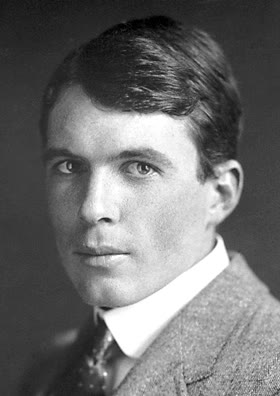
\includegraphics[width=\linewidth]{images/book4/bragg-wl.jpg}\par
{\footnotesize 威廉·劳伦斯·布拉格。}
\end{minipage}
\end{history}

\section{练习}

\begin{exercise}[$\star$]\label{exo:b3:x-ray-diffraction:1}
% ledger: lat:NaCl
对 \ce{NaCl}（$a = \qty{564.06}{pm}$），计算 $d_{111}$、$d_{200}$ 和 $d_{220}$。
\end{exercise}

\begin{exercise}[$\star$]\label{exo:b3:x-ray-diffraction:2}
% ledger: lat:Cu, xray:CuKa1
铜为面心立方结构，$a = \qty{361.50}{pm}$。用 Cu K$\alpha_1$（$\lambda = \qty{154.06}{pm}$），
先命名其前两个反射，再计算它们的 $2\theta$。
\end{exercise}

\begin{exercise}[$\star$]\label{exo:b3:x-ray-diffraction:3}
对于立方 P、I 和 F 点阵，下列反射 100、110、111、200、210、211、220 中
哪些是存在的？
\end{exercise}

\begin{exercise}[$\star$]\label{exo:b3:x-ray-diffraction:4}
给出边长分别为
$a$ 和 $b$ 的二维矩形点阵的倒格基，并画出前几个倒格点。
\end{exercise}

\begin{exercise}[$\star\star$]\label{exo:b3:x-ray-diffraction:5}
% ledger: lat:W
某金属在 $2\theta = 40.27$、58.26、73.20、87.01 和 \ang{100.66} 处出现谱线，
所用辐射为 Cu K$\alpha_1$。标定该图谱，求出点阵类型及 $a$。
\end{exercise}

\begin{exercise}[$\star\star$]\label{exo:b3:x-ray-diffraction:6}
% ledger: lat:KCl
一块 \ce{KCl} 晶体（$a = \qty{629.29}{pm}$）的实测密度为
\qty{1.99}{g/cm^3}（题中数据）。求 $Z$。
\end{exercise}

\begin{exercise}[$\star\star$]\label{exo:b3:x-ray-diffraction:7}
\ce{NaCl} 纳米粉末的 (200) 谱线（$2\theta = \ang{31.70}$）宽度为 \ang{0.40}，
仪器的贡献可忽略。估算微晶尺寸。
\end{exercise}

\begin{exercise}[$\star\star$]\label{exo:b3:x-ray-diffraction:8}
\ce{CsCl} 的 P 晶胞中，\ce{Cs+} 位于 $(0,0,0)$，\ce{Cl-} 位于 $(\frac12,\frac12,\frac12)$。取 $f
\approx$ 电子数，计算 $F_{100}$ 和 $F_{110}$ 以及它们
强度之比（仅考虑\omterm{def:b3:x-ray-diffraction:structure-factor}{结构因子}）。为什么 \ce{CsCl} 不是体心的？
\end{exercise}

\begin{exercise}[$\star\star$]\label{exo:b3:x-ray-diffraction:9}
证明：C 心点阵（附加格点位于 $(\frac12,\frac12,0)$）使
$h + k$ 为奇数的反射\omterm{def:b3:x-ray-diffraction:absence}{系统消光}。
\end{exercise}

\begin{exercise}[$\star\star\star$]\label{exo:b3:x-ray-diffraction:10}
解释为何 20 世纪 80 年代发现的合金，其衍射图样呈现尖锐的
十重对称斑点，并不与晶体学限制相矛盾，
以及它对晶体的定义有何改变。
\end{exercise}

\begin{exercise}[$\star\star\star$]\label{exo:b3:x-ray-diffraction:11}
证明：在 \textit{P}$2_1/c$ 中，\omterm{def:b3:x-ray-diffraction:space-group}{滑移面}使 $h0l$ 反射中
$l$ 为奇数的反射消光。
\end{exercise}

\begin{exercise}[$\star\star\star$]\label{exo:b3:x-ray-diffraction:12}
纯的对映异构体永远不能在含有
\omterm{def:b3:point-groups:inversion}{反演中心}、\omterm{def:b3:point-groups:mirror}{镜面}或\omterm{def:b3:x-ray-diffraction:space-group}{滑移面}的\omterm{def:b3:x-ray-diffraction:space-group}{空间群}中结晶。为什么？它被限定于哪类\omterm{def:b3:x-ray-diffraction:space-group}{空间群}，
弗里德尔定律在确定其绝对
构型时意味着什么？
\end{exercise}

% keep the heading with its problem box, which fills a page by itself
\clearpage
\enlargethispage{3\baselineskip}
\section{问题：哪一种白色粉末？}

\begin{problem}[{周末问题——未知立方盐的粉末图谱：
晶面间距、标定、晶胞参数和该盐的身份，以及
其微晶的尺寸}]
\label{pb:b3:x-ray-diffraction:1}
% ledger: xray:CuKa1, lat:NaCl, lat:KCl, lat:KBr
一种未知的白色晶态粉末，已知为 \ce{NaCl}、\ce{KCl} 或 \ce{KBr} 之一，
在 Cu K$\alpha_1$ 辐射（$\lambda = \qty{154.059}{pm}$）下给出以下谱线（题中数据，
为本题计算所得）：
\begin{center}\small
\begin{tabular}{lcccccc}
\hline
$2\theta$ / 度 & 28.342 & 40.512 & 50.178 & 58.632 & 66.380 & 73.692 \\
相对强度 & 100 & 92 & 38 & 20 & 61 & 49 \\ \hline
\end{tabular}
\end{center}
在 20 与 \ang{75} 之间未出现其他谱线。参考晶胞参数：
\ce{NaCl} \qty{564.06}{pm}、\ce{KCl} \qty{629.29}{pm}、\ce{KBr} \qty{658.47}{pm}。摩尔质量：
K 39.1、Na 23.0、Cl 35.5、Br \qty{79.9}{g/mol}。

\medskip\noindent\textbf{第一部分——\omterm{def:b3:x-ray-diffraction:miller}{晶面间距}。}
\begin{enumerate}
  \item 计算第一条谱线的 $\theta$ 和 $d$。
  \item 计算所有谱线的 $d$。
  \item 计算比值 $\sin^2\theta/\sin^2\theta_1$。
  \item 你发现了怎样的整数数列？
  \item 该图谱能否属于简单立方点阵？若能，$a$ 为多少？
  \item 对于简单立方点阵，哪个整数 $N$ 永远不可能出现？
        至此图谱能否区分这两种解释？
\end{enumerate}

\medskip\noindent\textbf{第二部分——实际点阵。}
\begin{enumerate}[resume]
  \item 三个候选均为 F 点阵。用 F 系列对谱线指标化。
  \item 由第一条谱线推出 $a$。
  \item 哪个候选符合？
  \item 对于该盐，为何全奇数反射 (111)、(311) 缺失？
  \item \ce{NaCl} 会出现 (111) 吗？\ce{KBr} 呢？
  \item 解释为何第一部分的简单点阵解释是一个陷阱。
\end{enumerate}

\medskip\noindent\textbf{第三部分——密度与组成。}
\begin{enumerate}[resume]
  \item 该晶胞含有多少个化学式单元？
  \item 由晶胞计算密度。
  \item 给出每种离子的配位数。
  \item 计算最短的 K--Cl 距离。
  \item 在 \ang{75} 以上，哪条反射会首先出现？
  \item 为何在鉴定物相时，强度不如峰位有用？
\end{enumerate}

\medskip\noindent\textbf{第四部分——精修与微晶尺寸。}
\begin{enumerate}[resume]
  \item 为何晶格参数最好由高角度谱线计算？
  \item 由 (420) 谱线计算 $a$。
  \item (420) 谱线在 $2\theta$ 中的宽度为 \ang{0.25}（仪器宽度
        可忽略）。估算微晶尺寸。
  \item 微晶尺寸为 \qty{1}{\micro m} 时，谱线会明显展宽吗？
  \item 给出结论：由 (420) 谱线精修得到的晶格参数，
        以及该粉末的物相。
\end{enumerate}
\end{problem}
